\iffalse
\documentclass[journal,12pt,twocolumn]{IEEEtran}
\usepackage{setspace}
\usepackage{gensymb}
\singlespacing
\usepackage[cmex10]{amsmath}
\usepackage{amsthm}
\usepackage{mathrsfs}
\usepackage{txfonts}
\usepackage{stfloats}
\usepackage{bm}
\usepackage{cite}
\usepackage{cases}
\usepackage{subfig}
\usepackage{longtable}
\usepackage{multirow}
\usepackage{enumitem}
\usepackage{mathtools}
\usepackage{steinmetz}
\usepackage{tikz}
\usepackage{circuitikz}
\usepackage{verbatim}
\usepackage{tfrupee}
\usepackage[breaklinks=true]{hyperref}
\usepackage{tkz-euclide}
\usetikzlibrary{calc,math}
\usepackage{listings}
    \usepackage{color}                                            %%
    \usepackage{array}                                            %%
    \usepackage{longtable}                                        %%
    \usepackage{calc}                                             %%
    \usepackage{multirow}                                         %%
    \usepackage{hhline}                                           %%
    \usepackage{ifthen}                                           %%
  %optionally (for landscape tables embedded in another document): %%
    \usepackage{lscape}     
\usepackage{multicol}
\usepackage{chngcntr}
\DeclareMathOperator*{\Res}{Res}
\renewcommand\thesection{\arabic{section}}
\renewcommand\thesubsection{\thesection.\arabic{subsection}}
\renewcommand\thesubsubsection{\thesubsection.\arabic{subsubsection}}

\renewcommand\thesectiondis{\arabic{section}}
\renewcommand\thesubsectiondis{\thesectiondis.\arabic{subsection}}
\renewcommand\thesubsubsectiondis{\thesubsectiondis.\arabic{subsubsection}}

% correct bad hyphenation here
\hyphenation{op-tical net-works semi-conduc-tor}
\def\inputGnumericTable{}                                 %%

\lstset{
frame=single, 
breaklines=true,
columns=fullflexible
}

\begin{document}


\newtheorem{theorem}{Theorem}[section]
\newtheorem{problem}{Problem}
\newtheorem{proposition}{Proposition}[section]
\newtheorem{lemma}{Lemma}[section]
\newtheorem{corollary}[theorem]{Corollary}
\newtheorem{example}{Example}[section]
\newtheorem{definition}[problem]{Definition}
\newcommand{\BEQA}{\begin{eqnarray}}
\newcommand{\EEQA}{\end{eqnarray}}
\newcommand{\define}{\stackrel{\triangle}{=}}

\bibliographystyle{IEEEtran}
\providecommand{\mbf}{\mathbf}
\providecommand{\pr}[1]{\ensuremath{\Pr\left(#1\right)}}
\providecommand{\qfunc}[1]{\ensuremath{Q\left(#1\right)}}
\providecommand{\sbrak}[1]{\ensuremath{{}\left[#1\right]}}
\providecommand{\lsbrak}[1]{\ensuremath{{}\left[#1\right.}}
\providecommand{\rsbrak}[1]{\ensuremath{{}\left.#1\right]}}
\providecommand{\brak}[1]{\ensuremath{\left(#1\right)}}
\providecommand{\lbrak}[1]{\ensuremath{\left(#1\right.}}
\providecommand{\rbrak}[1]{\ensuremath{\left.#1\right)}}
\providecommand{\cbrak}[1]{\ensuremath{\left\{#1\right\}}}
\providecommand{\lcbrak}[1]{\ensuremath{\left\{#1\right.}}
\providecommand{\rcbrak}[1]{\ensuremath{\left.#1\right\}}}
\theoremstyle{remark}
\newtheorem{rem}{Remark}
\newcommand{\sgn}{\mathop{\mathrm{sgn}}}
\providecommand{\abs}[1]{\left\vert#1\right\vert}
\providecommand{\res}[1]{\Res\displaylimits_{#1}} 
\providecommand{\norm}[1]{\left\lVert#1\right\rVert}
\providecommand{\mtx}[1]{\mathbf{#1}}
\providecommand{\mean}[1]{E\left[ #1 \right]}
\providecommand{\fourier}{\overset{\mathcal{F}}{ \rightleftharpoons}}
\providecommand{\system}{\overset{\mathcal{H}}{ \longleftrightarrow}}
\newcommand{\solution}{\noindent \textbf{Solution: }}
\newcommand{\cosec}{\,\text{cosec}\,}
\providecommand{\dec}[2]{\ensuremath{\overset{#1}{\underset{#2}{\gtrless}}}}
\newcommand{\myvec}[1]{\ensuremath{\begin{pmatrix}#1\end{pmatrix}}}
\newcommand{\mydet}[1]{\ensuremath{\begin{vmatrix}#1\end{vmatrix}}}
\numberwithin{equation}{subsection}
\makeatletter
\@addtoreset{figure}{problem}
\makeatother

\let\StandardTheFigure\thefigure
\let\vec\mathbf
\renewcommand{\thefigure}{\theproblem}



\def\putbox#1#2#3{\makebox[0in][l]{\makebox[#1][l]{}\raisebox{\baselineskip}[0in][0in]{\raisebox{#2}[0in][0in]{#3}}}}
     \def\rightbox#1{\makebox[0in][r]{#1}}
     \def\centbox#1{\makebox[0in]{#1}}
     \def\topbox#1{\raisebox{-\baselineskip}[0in][0in]{#1}}
     \def\midbox#1{\raisebox{-0.5\baselineskip}[0in][0in]{#1}}

\vspace{3cm}


\title{Assignment 1}
\author{Jaswanth Chowdary Madala}





% make the title area
\maketitle

\newpage

%\tableofcontents

\bigskip

\renewcommand{\thefigure}{\theenumi}
\renewcommand{\thetable}{\theenumi}


\begin{enumerate}
%\begin{figure}[ht]
%\centering
%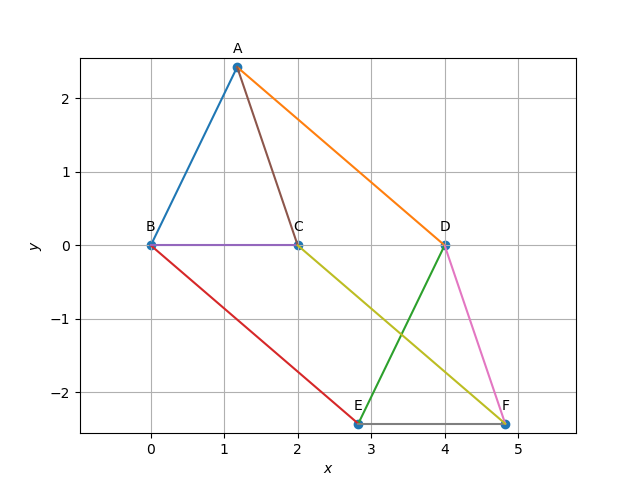
\includegraphics[width = \columnwidth]{"./chapters/11/11/4/13/figs/fig.png"}
%\caption{Graph}
%\label{fig:chapters/11/11/4/13/1}
%\end{figure}

\textbf{Solution:}
\fi
The equation of the conic with focus $\vec{F}$, directrix $\vec{n}^\top\vec{x} = c$ and eccentricity $e$ is given by
\begin{align}
\vec{x}^\top\vec{V}\vec{x} + 2\vec{u}^\top\vec{x} + f = 0
\label{eq:chapters/11/11/4/13/1}
\end{align}
where
\begin{align}
\vec{V} &\triangleq \norm{\vec{n}}^2\vec{I} - e^2\vec{n}\vec{n}^\top \label{eq:chapters/11/11/4/13/2} \\
\vec{u} &\triangleq ce^2\vec{n} - \norm{\vec{n}}^2\vec{F} \label{eq:chapters/11/11/4/13/3} \\
f &\triangleq \norm{\vec{n}}^2\norm{\vec{F}}^2 - c^2e^2 \label{eq:chapters/11/11/4/13/4}
\end{align}
also
\begin{align}
f_0 &= \vec{u}^\top\vec{V}^{-1}\vec{u} - f\\
l &= 2\frac{\sqrt{\abs{f_0\lambda_2}}}{\lambda_1}
\end{align}

\begin{enumerate}
\item $\vec{n}$: Given that the conic has foci as
\begin{align}
\vec{F_1} &= \myvec{4\\0}\\
\vec{F_2} &= \myvec{-4\\0}
\end{align}
The direction vector of $F_1F_2$ is given by
\begin{align}
\vec{m} &= \vec{F_1} - \vec{F_2}\\
&= \myvec{1\\0}
\end{align}
Hence the normal to the directrix is given by,
\begin{align}
\vec{n} = \myvec{1\\0}
\end{align}

\item $\vec{u}$: The centre of the conic is given by
\begin{align}
\vec{c} &= \frac{\vec{F_1} + \vec{F_2}}{2}
\end{align}
\begin{align}
\vec{c} &= \myvec{0\\0}\\
\vec{c} &= -\vec{V}^{-1}\vec{u}
\label{eq:chapters/11/11/4/13/5}
\end{align}
Since $\vec{c} = \vec{0}$ and $\vec{V}^{-1} \neq \vec{0}$, it follows from \eqref{eq:chapters/11/11/4/13/5} that 
\begin{align}
\vec{u} = \myvec{0\\0}
\end{align}

From the above expressions we get
\begin{align}
\vec{V} &= \myvec{1-e^2&0\\0&1} \label{eq:chapters/11/11/4/13/6} \\
\vec{F} &= \myvec{ce^2\\0} \label{eq:chapters/11/11/4/13/7}\\
f &= c^2e^2\brak{e^2-1} \label{eq:chapters/11/11/4/13/8}\\
f_0 &= - f \label{eq:chapters/11/11/4/13/9}\\
l &= 2\frac{\sqrt{\abs{f\lambda_2}}}{\lambda_1}\label{eq:chapters/11/11/4/13/10}
\end{align}

From equation \eqref{eq:chapters/11/11/4/13/6} the eigen values of matrix $\vec{V}$ - $\lambda_1, \lambda_2$ are given by,
\begin{align}
\lambda_1 &= 1-e^2
\label{eq:chapters/11/11/4/13/11}\\
\lambda_2 &= 1
\label{eq:chapters/11/11/4/13/12}
\end{align}

From equation \eqref{eq:chapters/11/11/4/13/7} we get,
\begin{align}
ce^2 = 4 \label{eq:chapters/11/11/4/13/13}
\end{align}
\item Eccentricity: Given that the conic has the latus rectum length 12. Substituting the expressions of $\lambda_1,\lambda_2$ from the equations \eqref{eq:chapters/11/11/4/13/11}, \eqref{eq:chapters/11/11/4/13/12} in \eqref{eq:chapters/11/11/4/13/10} gives
\begin{align}
l = \frac{2ce}{\sqrt{e^2-1}} &= 12\\
\frac{ce}{\sqrt{e^2-1}} &= 6
\end{align}
Substitute the expression of $c$ from \eqref{eq:chapters/11/11/4/13/13} gives,
\begin{align}
\frac{4}{e\sqrt{e^2-1}} &= 6
\end{align}
Squaring on both sides gives,
\begin{align}
9e^2\brak{e^2-1} &= 4\\
9e^4-9e^2-4 &= 0
\label{eq:chapters/11/11/4/13/14}
\end{align}
The equation \eqref{eq:chapters/11/11/4/13/14} is a quadratic equation in $e^2$.
Solving it gives two roots one of which is negative, as $e^2$ is positive we have
\begin{align}
%e^2 &= \frac{-\brak{-9}\pm\sqrt{\brak{-9}^2-4\times9\times\brak{-4}}}{2\times9}\\
e^2 &= \frac{4}{3}
\end{align}
From equation \eqref{eq:chapters/11/11/4/13/8}, \eqref{eq:chapters/11/11/4/13/13}, we get
\begin{align}
f = 4
\end{align} 
\end{enumerate}
The equation of the conic is given by
\begin{align}
\vec{x}^\top\myvec{-\frac{1}{3}&0\\0&1}\vec{x} +4 = 0
\end{align}
\begin{figure}[ht]
\centering
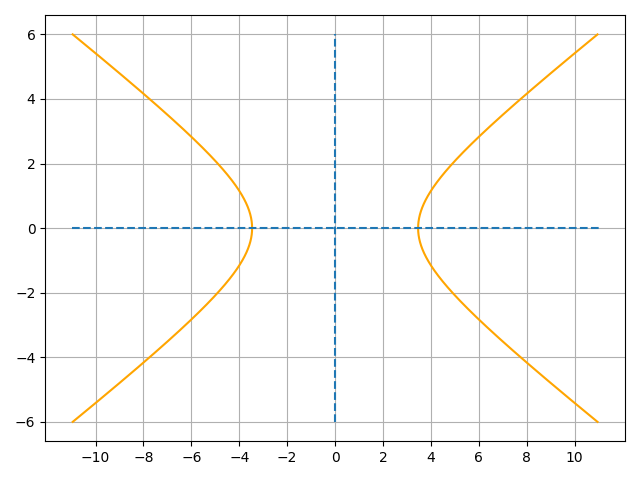
\includegraphics[width = \columnwidth]{chapters/11/11/4/13/figs/fig1.png}
\caption{Graph}
\label{fig:chapters/11/11/4/13/1}
\end{figure}
\begin{table}[h]
\centering
%%%%%%%%%%%%%%%%%%%%%%%%%%%%%%%%%%%%%%%%%%%%%%%%%%%%%%%%%%%%%%%%%%%%%%
%%                                                                  %%
%%  This is a LaTeX2e table fragment exported from Gnumeric.        %%
%%                                                                  %%
%%%%%%%%%%%%%%%%%%%%%%%%%%%%%%%%%%%%%%%%%%%%%%%%%%%%%%%%%%%%%%%%%%%%%%

\begin{center}
\begin{tabular}{|c|c|c|}
\hline
\textbf{Parameter}& \textbf{Description} &\textbf{Value}\\ \hline
$\vec{F_1}$		 &	Focus 1 of hyperbola&$\myvec{4\\0}$\\ \hline
$\vec{F_2}$		 &	Focus 2 of hyperbola&$\myvec{-4\\0}$\\ \hline
$l$		 &  Length of latus rectum&12 \\ \hline
\end{tabular}
\end{center}

\caption{}
\label{tab:chapters/11/11/4/13/1}
\end{table}
